% Chapter Template

\chapter{Introduction} % Main chapter title

\label{chap:intro} % Change X to a consecutive number; for referencing this chapter elsewhere, use \ref{ChapterX}



Understanding the physics behind interstellar PUI is of special interest as they give us a possibility to directly observe properties of the interstellar medium by in-situ measurements within the heliosphere. 
Additionally, the observation of their VDF helps us to understand interplanetary transport as the evolution of their characteristic VDF shows signatures of the transport processes involved.
\begin{figure}[h]
	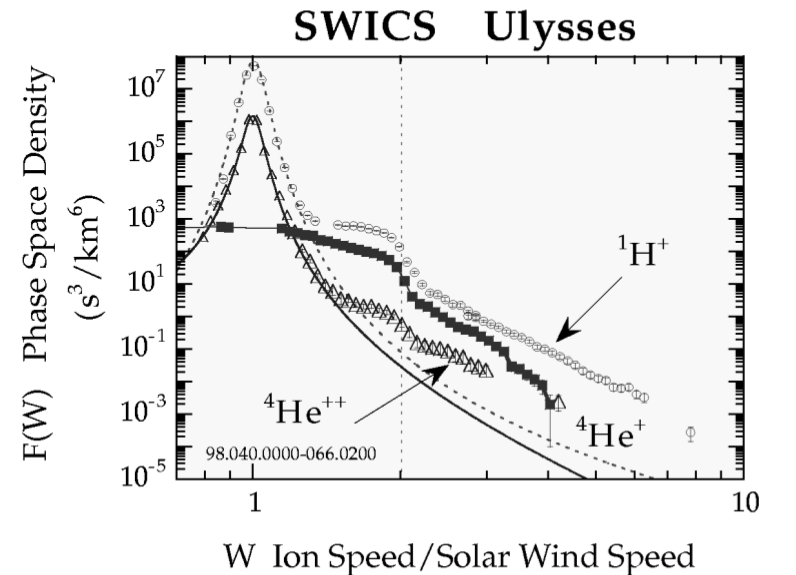
\includegraphics[width=0.8\textwidth]{Figures/sw_pui_gloeckler.png}
	\centering
	\caption{Phase space density for $\mathrm{He^{2+}}$, $\mathrm{He^{+}}$ and $\mathrm{H^{+}}$ against $w = \frac{v_\mathrm{ion}}{v_\mathrm{sw}}$ in the slow solar wind ($v_\mathrm{sw} = 375\,\mathrm{km\,s^{-1}}$). PUI distributions are clearly visible for all three species in the $w$ range between $\sim$ 1.5 and 2 followed by a cutoff at $w = 2$ and high-velocity tails. Solar wind distributions are represented by the dashed and solid curves for $\mathrm{He^{2+}}$ and $\mathrm{H^{+}}$. The figure is taken from \citet{gloeckler1999}.} 
	\label{fig:gloeckler}
\end{figure}
Many studies on PUI VDF base on measurements of Ulysses SWICS \citep{gloeckler_geiss}.
These studies were limited to 1D reduced observations in the spacecraft frame until today, as only the absolute values of velocities were considered.
An example by \citet{gloeckler1999} is shown in Fig. \ref{fig:gloeckler}. Here we see the phase space density of three different pickup ion species drawn against $w$, which is the ion's velocity divided by the current solar wind speed. The pickup ions shows a non-Maxwellian distribution with a clear cutoff at w=2. While the distributions of He2+ and H+ are superimposed by the distribution of the solar wind ions around w=1, the distribution of He+ PUI is unveiled.  
However, the actual PUI VDF is multi-dimensional and cannot be reproduced from the reduced 1D measurement without making assumptions on the underlying distribution.
Several 3D VDF may lead to the same 1D VDF when being reduced and thus every 1D measurement is ambiguous.

As Ulysses SWICS is capable of resolving the inflow direction of incident ions, a three-dimensional VDF can be obtained when taking into account all given information.
The aim of this thesis is to make use of this information and to develop a tool to provide three-dimensional VDFs. 
PUI differ from solar wind ions by a non-Maxwellian VDF. As this distribution is particularly broad, He+ PUI are the perfect candidates for testing the tool and for being studied with it.
\\
The thesis starts with an introduction into PUI, before the Ulysses mission and the instrument SWICS with its measurement principle are described. In the third chapter a virtual detector is developed to translate the raw He+ data into three-dimensional velocity components. For this, SWICS' intrigue geometry has to be considered as well as Ulysses' orientation in space and its eigen-velocity. In the final section the obtained three-dimensional spectra are presented in different projections.



%%%
%-------------------------------------------------------------
%%%
